\chapter{Results and Discussion}

%%%%%%%%%%%%%%%%%%%%%%%%%%%%%%%%%%%%%%%%%%%%%%%%%%%%%%%%%%%%%%%%%%%%%%%%
\section{Final Numbers}
% crex: https://docs.google.com/spreadsheets/d/154c_FlXKs06Dbn1UEjuJeL52RLanBTXx/edit#gid=1377286011

\begin{comment}
    Measured asymmetry 
    $\downarrow$
    correct for Coulomb distortions 
    $\downarrow$
    Weak density at one $Q^2$
    $\downarrow$
    small correction for $G_E^n$, $G_E^s$
    $\downarrow$
    Neutron density at one $Q^2$
    $\downarrow$
    assume surface thickness good to 25\% (MFT)
    $\downarrow$
    $R_n$

\end{comment}
The overall beam polarization is determined by calculating the inverse-variance 
weighted average of the Compton and Moller measurements.
\begin{table}[!h]
    % PREX-II Compton
    % PREX-II Moller: https://prex.jlab.org/DocDB/0004/000468/003/DNP_Oct2020.pdf
    % CREX Compton: AJZ thesis
    % CREX Moller: AJZ thesis
    \centering
    \begin{tabular}{c | c c}
	\hline
	    & PREX-II	& CREX	\\
	\hline
	Compton	& ($89.68 \pm 0.15$)\%  & ($87.115 \pm 0.453$)\%	\\
	Moller	& ($89.67 \pm 0.80$)\%	& ($87.06 \pm 0.74$)\%  \\
	\hline
	Average	& ($89.7 \pm 0.8$)\%	& ($87.10 \pm 0.39$)\%	\\
	\hline
    \end{tabular}
    \caption{Beam polarization measured by the Compton and Moller polarimeters.}
\end{table}

%%%%%%%%%%%%%%%%%%%%%%%%%%%%%%%%%%%%%%%%%%%%%%%%
% \subsection{Asymmetry}
After applying the beam false asymmetry correction described in chapter~\ref{cha:data_analysis} and
identifying various background asymmetries in chapter~\ref{cha:systematic_uncertainties}, 
the blinded PV asymmetry will be extracted using Eq. \ref{eq:background_correction}, 
which we restate here:
\begin{equation*}
    \CA_{\text{PV}} = \frac{\CA_{\text{cor}}/\CP - \sum_i \CA_i f_i}{1 - \sum_i f_i}
\end{equation*}
The list of various corrections to the final result are shown in 
Table~\ref{tab:prex_corrections} and \ref{tab:crex_corrections}.

\begin{table}[!h]
    \centering
    \begin{tabular}{l r@{ $\pm$ }l r@{ $\pm$ }l}
	\hline
	Correction & \multicolumn{2}{c}{Absolute (ppb)}	& \multicolumn{2}{c}{Relative (\%)}   \\
	\hline
	Beam trajectory and energy  & -60.4	& 3.0	& 11.0	& 0.5	\\ 
	Charge correction           & 20.7	& 0.2   & 3.8	& 0.0   \\ 
	\hline
	Beam polarization           & 56.8	& 5.2   & 10.3	& 1.0   \\ 
	Target diamond foils        & 0.7	& 1.4   & 0.1	& 0.3   \\ 
	Spectrometer rescattering   & 0.0	& 0.1   & 0.0  	& 0.0   \\ 
	Inelastic contributions     & 0.0	& 0.1   & 0.0  	& 0.0   \\ 
	Transverse asymmetry        & 0.0	& 0.3   & 0.0  	& 0.1   \\ 
	Detector nonlinearity       & 0.0	& 2.7   & 0.0  	& 0.5   \\ 
	Angle determination         & 0.0	& 3.5   & 0.0  	& 0.6   \\ 
	Acceptance function         & 0.0	& 2.9   & 0.0  	& 0.5   \\ 
	\hline
	Total correction	    & 17.7	& 8.2	& 3.2	& 1.5	\\
	Statistical uncertainty	    & \multicolumn{2}{c}{16}	& \multicolumn{2}{c}{2.9}   \\
	\hline
    \end{tabular}
    \caption{Corrections and corresponding systematic uncertainties to $\CA_{\text{PV}}$ in PREX-II.}
    \label{tab:prex_corrections}
\end{table}

\begin{table}[!h]
    \centering
    \begin{tabular}{l r@{ $\pm$ }l r@{ $\pm$ }l}
	\hline
	Correction & \multicolumn{2}{c}{Absolute (ppb)}	& \multicolumn{2}{c}{Relative (\%)}   \\
	\hline
	Beam trajectory and energy  & 68  & 7     & 2.5	    & 0.3   \\         
	Beam charge asymmetry       & 112 & 1     & 4.2     & 0.0   \\         
	\hline
	Beam polarization	    & 382 & 13    & 14.3    & 0.5   \\         
	Isotopic purity             & 19  & 3     & 0.7     & 0.1   \\         
	3.831 MeV ($2^+$) inelastic & -35 & 19    & -1.3    & 0.7   \\         
	4.507 MeV ($3^-$) inelastic & 0   & 10    & 0	    & 0.4   \\ 
	5.370 MeV ($3^-$) inelastic & -2  & 4     & -0.1    & 0.1   \\         
	Transverse asymmetry        & 0   & 13    & 0	    & 0.5   \\ 
	Detector nonlinearity       & 0   & 7     & 0	    & 0.3   \\         
	Acceptance                  & 0   & 24    & 0  	    & 0.9   \\         
	Radiative corrections	    & 0   & 10    & 0  	    & 0.4   \\         
	\hline
	Total systematic uncertainty	& \multicolumn{2}{c}{40}    & \multicolumn{2}{c}{1.5}	\\
	Statistical uncertainty		& \multicolumn{2}{c}{106}   & \multicolumn{2}{c}{4.0}	\\
	\hline
    \end{tabular}
    \caption{Corrections and corresponding systematic uncertainties to $\CA_{\text{PV}}$ in CREX.}
    \label{tab:crex_corrections}
\end{table}

The last step is unblinding, in which we subtract $\CA_{\text{blind}}$ from the blinded
$\CA_{\text{PV}}$. The blinding factor is a secret value that is randomly generated 
from a $\pm900$~ppb box, this secret value is 
added to each helicity quadruplet (octuplet) asymmetry by the JAPAN analyzer. 
Surprisingly, the value of $\CA_{\text{blind}}$ for PREX-II is very close to 0, 
resulting in the unblinded $\CA_{\text{PV}}$ being almost the same as the blinded value. 
The final asymmetry values are presented in Table~\ref{tab:pcrex_final_number}.
\begin{table}[!h]
    \centering
    \begin{tabular}{c | c c}
	\hline
	Asymmetry   & PREX-II	& CREX	\\
	\hline
	$\CA_{\text{raw}}$ & $431.64 \pm 44.01$    & $2106 \pm 178.9$	\\
	$\CA_{\text{cor}}$ & $492.02 \pm 13.52$    & $2080.3 \pm 83.8$	\\
	Blinded $\CA_{\text{PV}}$ & $549.4 \pm 16.1 \pm 8.1$    & $2412.3 \pm 106.1 \pm 38.7$	\\
	$\CA_{\text{blind}}$	& -0.5	& -255.7    \\
	\hline
	Unblinded $\CA_{\text{PV}}$	& $550 \pm 16 \pm 8$	& $2668 \pm 106 \pm 40$	\\
	\hline
    \end{tabular}
    \caption{The path to a physical PV asymmetry. All values are in units of ppb.}
    \label{tab:pcrex_final_number}
\end{table}

%%%%%%%%%%%%%%%%%%%%%%%%%%%%%%%%%%%%%%%%%%%%%%%%
\subsection{Neutron Skin Thickness}
\label{subsec:neutron_skin_thickness}
With the physical PV asymmetry, the weak FF is calculated using Eq.~\ref{eq:asymmetry}.
\begin{equation}
    F_W ({}^{208}\text{Pb}) = 0.368  \pm 0.013 \ (\text{exp}) \pm 0.001 \ (\text{theo})
\end{equation}
Here the experimental uncertainty incorporates both statistical and systematic contributions.

The experimental value of the weak radius is determined from the correlation between the weak radius and PV asymmetry. In the correlation plot, the weak radius corresponding to the measured PV asymmetry is obtained as the experimental value. Similarly, the neutron skin thickness is derived using the same approach.

The correlation plot is generated by fitting the weak charge densities, which are
predicted by a wide range of DFT models, to a two-parameter Fermi function. 
By knowing the weak charge density function, the corresponding PV asymmetry and
weak radius can be identified for each model, as shown in Fig.~\ref{fig:prex_Rw}.
The two-parameter Fermi function has been discussed in Sec.~\ref{subsec:models}.
\begin{equation*}
    \rho_W(r) = \rho_W^0 \frac{\sinh(c/a)}{\cosh(r/a) + \cosh(c/a)}
\end{equation*}
here $c$ denotes the nuclear size and $a$ describes the surface thickness. 

\begin{figure}[!h]
    \centering
    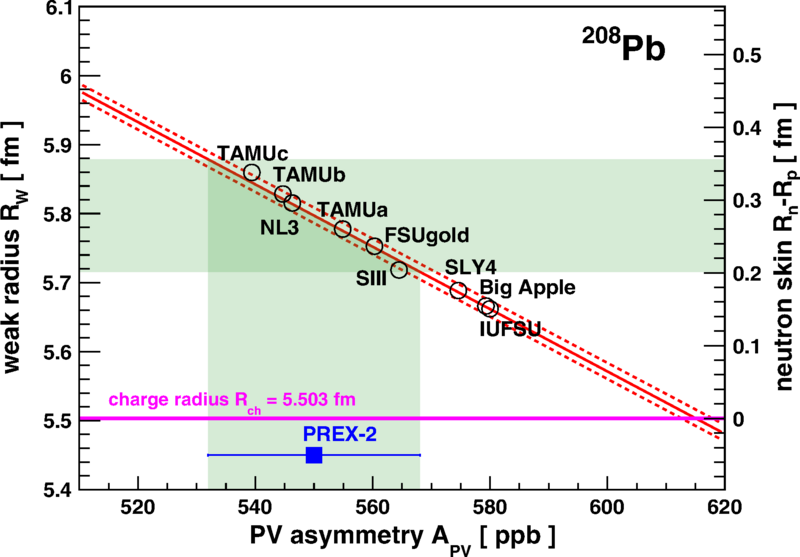
\includegraphics[width=0.6\linewidth]{prex_Rw}
    \caption[Correlation between the weak radius/neutron skin thickness and $\CA_{\text{PV}}$]
    {Correlation between the weak radius (left vertical axis) or neutron skin thickness 
    (right vertical axis) and $\CA_{\text{PV}}$ for \Pb, as predicted by a series 
    of DFT models \cite{PhysRevLett.126.172502}. 
    The red solid line describes the fitted correlation based on the predictions of
    the DFT models, the red dashed line and the green band indicate the 1-$\sigma$ uncertainty 
    for the correlation and measured values, respectively.}
    \label{fig:prex_Rw}
\end{figure}

% The fits suggest \cite{PhysRevLett.126.172503}:
% \begin{equation}
%     a = 0.605 \pm 0.025\ \mathrm{fm}
% \end{equation}

The weak charge radius of \Pb is extracted to be:
\begin{equation}
    % R^2_W = \frac{1}{Q_W} \int r^2 \rho_W(r)d^3r = \frac{3}{5}c^2 + \frac{7}{5}(\pi a)^2
    R_W ({}^{208}\text{Pb}) = 5.795 \pm 0.082 \ (\text{exp}) \pm 0.013 \ (\text{theo})\ \mathrm{fm}
\end{equation}
and the neutron skin thickness of \Pb:
\begin{equation}
    R_{\text{skin}} ({}^{208}\text{Pb}) = R_n - R_p = 0.278 \pm 0.078 \ (\text{exp}) \pm 0.012 \ (\text{theo})\ \mathrm{fm}
\end{equation}

Similarly, the weak radius and neutron skin thickness of \Ca can be extracted,
as summarized in Table~\ref{tab:pcrex_neutron_skin}.
\begin{table}[!h]
    \centering
    \begin{tabular}{l | c c}
	\hline
	Exp	& PREX-II   & CREX  \\
	\hline
	Target	& \Pb	    & \Ca   \\
	$\langle Q^2 \rangle $ ($\mathrm{GeV}^2$)	& $ 0.00616 \pm 0.00005 $   & $0.0297 \pm 0.0002 $  \\
	$\langle \CA_{\text{PV}} \rangle$ (ppb)   & $550 \pm 16 \ (\text{stat}) \pm 8 \ (\text{syst})$	& $2668 \pm 106 \ (\text{stat}) \pm 40 \ (\text{syst})$ \\
	$F_W$	& $0.368 \pm 0.013 \ (\text{exp}) \pm 0.001 \ (\text{theo})$    & $0.1304 \pm 0.0052 \ (\text{stat}) \pm 0.0020 \ (\text{syst})$    \\
	$F_{ch} - F_W$	& $0.041 \pm 0.013 \ (\text{exp}) \pm 0.001 \ (\text{theo})$    & $0.0277 \pm 0.0052 \ (\text{stat}) \pm 0.0020 \ (\text{syst})$    \\
	$R_W$ (fm)	& $5.795 \pm 0.082 \ (\text{exp}) \pm 0.013 \ (\text{theo})$    & $3.640 \pm 0.026 \ (\text{exp}) \pm 0.023 \ (\text{theo})$\\
	$R_n - R_p$ (fm)  & $0.278 \pm 0.078 \ (\text{exp}) \pm 0.012 \ (\text{theo})$	& $0.121 \pm 0.026 \ (\text{exp}) \pm 0.024 \ (\text{theo})$    \\
	% $\rho_W^0$ ($\mathrm{fm}^{-3}$)	& $-0.0798 \pm 0.0038 \ (\text{exp}) \pm 0.0013 \ (\text{theo})$	&   \\
	% $\rho_b^0$ ($\mathrm{fm}^{-3}$)	& $0.1482 \pm 0.0040 $	&   \\
	\hline
    \end{tabular}
    \caption{Physical results extracted from PREX-II and CREX. 
    % The experimental uncertainty in PREX-II   
    }
    \label{tab:pcrex_neutron_skin}
\end{table}

Combining PREX-I and PREX-II results, the weak radius and the neutron skin are 
determined to be:
\begin{equation}
    \begin{gathered}
	R_W({}^{208}\text{Pb}) = 5.800 \pm 0.075\ \mathrm{fm}  \\
	R_{skin}({}^{208}\text{Pb}) = 0.283 \pm 0.71\ \mathrm{fm}   \\
    \end{gathered}
\end{equation}
%%%%%%%%%%%%%%%%%%%%%%%%%%%%%%%%%%%%%%%%%%%%%%%%
\subsection{Density Dependence of the Symmetry Energy}
In nuclear density functional theory, the neutron skin thickness of \Pb is 
correlated with the density dependence of the symmetry energy $L$. 
By plotting the predictions from DFT calculations using a set of energy density 
functionals, a linear correlation between $L$ and $R_{\text{skin}}$ can be established,
as demonstrated in Fig.~\ref{fig:L_vs_R_skin}. Using this correlation, we can determine
the symmetry energy slope $L$ that corresponds to our measured $R_{\text{skin}}$ in \Pb. 
The values of $L$ at the nuclear saturation density 
$\rho_0 \sim 0.15 \mathrm{fm}^{-3}$ and the nuclear density $\rho_1 \sim 0.15 \mathrm{fm}^{-3}$ 
are determined to be:
\begin{equation}
    L(\rho_0) = 106 \pm 37 \ \mathrm{MeV}	\qquad L(\rho_1) = 71.5 \pm 22.6 \ \mathrm{MeV}
\end{equation}
\begin{figure}[!h]
    \centering
    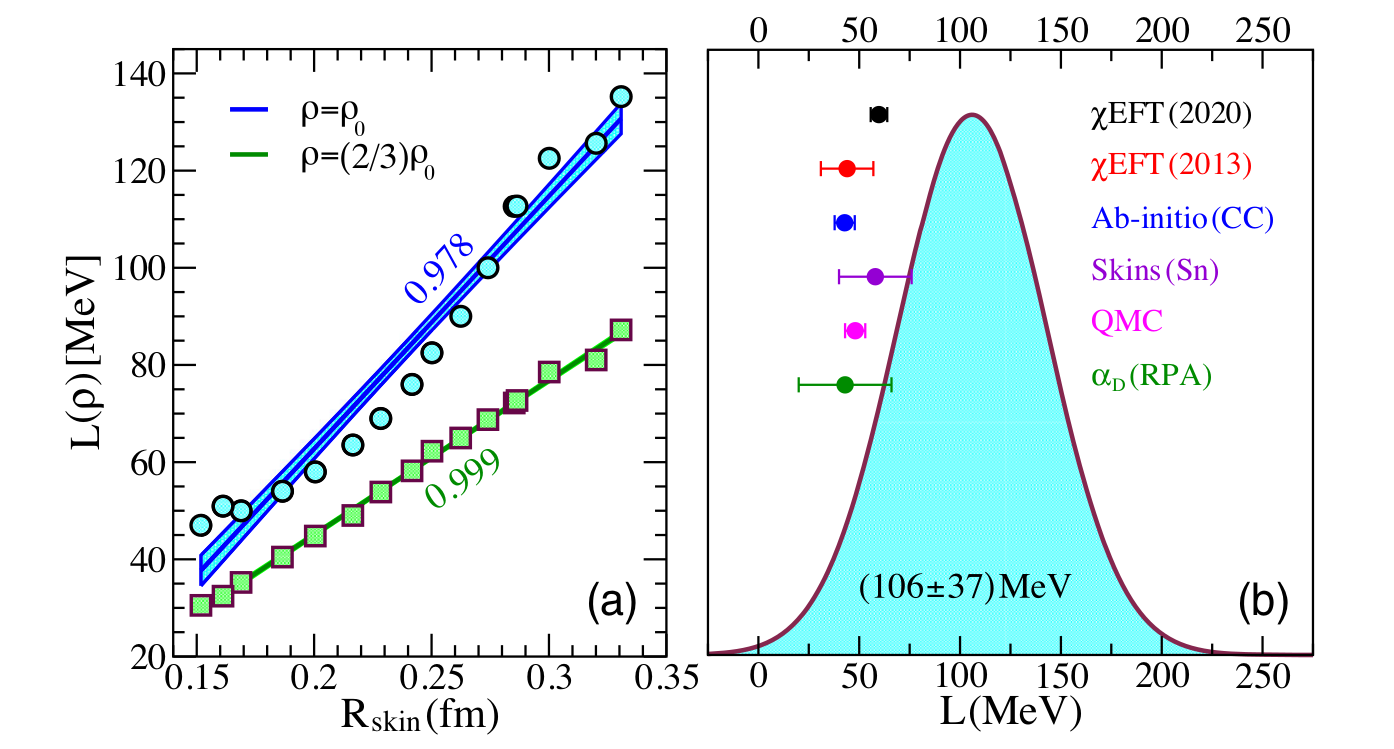
\includegraphics[width=0.6\linewidth]{L_vs_R_skin}
    \caption[Correlation plot between L and Rskin]
    {Left: correlation between the symmetry energy slope and the neutron skin thickness of \Pb.
    The blue line represents the correlation at the nuclear saturation density,
    while the green line represents the correlation at the nuclear density.
    The correlation coefficients are indicated by the numbers along the lines.
    Right: A Gaussian probability distribution for $L(\rho_0)$ inferred from 
    the correlation plot on the left. The six data points are theoretical
    predictions of $L(\rho_0)$ from different approaches \cite{PhysRevLett.126.172503}.
    }
    \label{fig:L_vs_R_skin}
\end{figure}
% the 0.28 fm neutron skin thickness of Pb208 is larger than the predicted
% value of 0.15-0.18 fm by most models. Such a thin neutron skin indicates
% a strong symmetry pressure, therefore a larger neutron star radius.
%%%%%%%%%%%%%%%%%%%%%%%%%%%%%%%%%%%%%%%%%%%%%%%%
\subsection{Difference Between the Charge and Weak Form Factors}
As discussed in subsection~\ref{subsec:neutron_skin_thickness}, the weak form factor
and weak radius are extracted through their correlations with the PV asymmetry,
while the correlation depends on the weak charge distribution function $\rho_W(r)$.
The model dependence of $F_W$ an $R_W$ arises from the choice of $\rho_W(r)$ to match the
measured $\CA_{\text{PV}}$. 

Unexpectly, for \Ca, the determination of $F_W$ at the reference momentum transfer
of $q = 0.8733\ \text{fm}^{-1}$ is insensitive to the shape of $\rho_W$ \cite{PhysRevLett.129.042501}. 
This indicates that the calculated value of $F_W$ and $F_{ch} - F_W$ have minimal
model dependence. Consequently, in Table~\ref{tab:pcrex_neutron_skin}, 
the entries for $F_W$ and $F_{ch} - F_W$ for \Ca have only experimental uncertainties, 
without any theoretical uncertainties.

On the other hand, the large theoretical uncertainty in $R_W$ for \Ca stems 
from the fact that the correlation equation between $F_W$ and $R_W$ -- 
$F_{ch}(q) - F_W(q) \approx q^2 (R^2_{W} - R^2_{ch})/6$ -- is only valid in
the limit of $q \rightarrow 0$, which is not applicable due to the large value of $q$ in CREX.

Therefore, for \Ca, $F_W$ and $F_{ch} - F_{W}$ are more reliable than $R_W$ and $R_W - R_{ch}$.
A comparison of $F_{ch} - F_W$ for \Ca between experimental result and theoretical predictions,
as shown in Fig.~\ref{fig:CREX_FF_difference}, 
reveals that various models overestimate the difference between the charge
and weak form factors for \Ca.

\begin{figure}[!h]
    \centering
    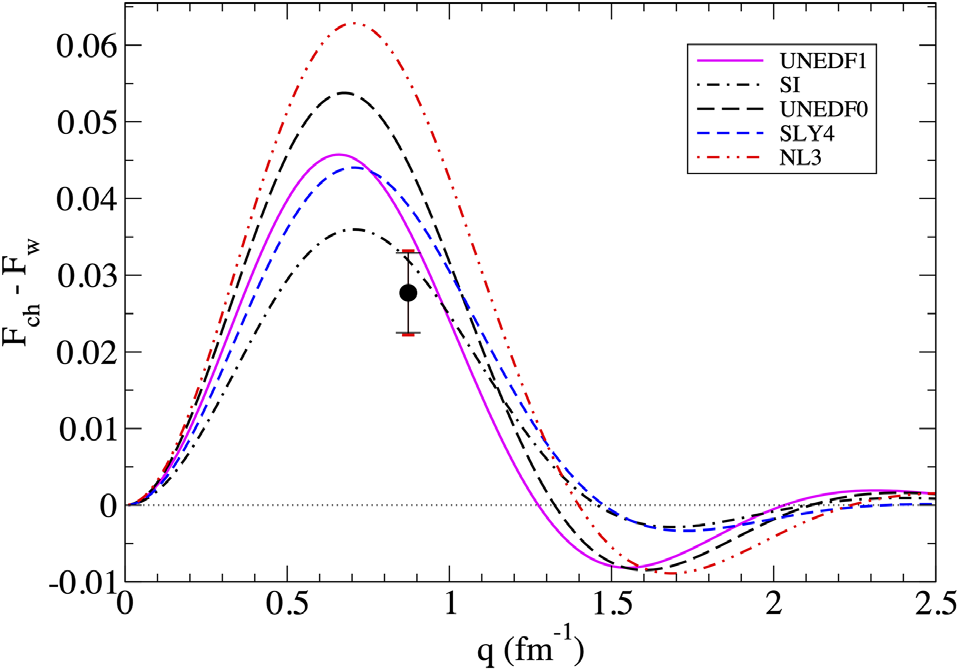
\includegraphics[width=0.6\linewidth]{CREX_FF_difference}
    \caption[The difference between the charge and weak FFs for \Ca.]
    { The difference between the charge and weak form factor for \Ca. The black
    point indicates the CREX measurement. The curves represent theoretical 
    predictions of $F_{ch} - F_W$ as a function of $q$ from a series of EDF modles,
    as listed in the legend.
    }
    \label{fig:CREX_FF_difference}
\end{figure}


%%%%%%%%%%%%%%%%%%%%%%%%%%%%%%%%%%%%%%%%%%%%%%%%%%%%%%%%%%%%%%%%%%%%%%%%
\section{Physical Implication}
\begin{comment}
    \begin{itemize}
	\item The \Pb radius constrains the pressure of neutron matter at subnuclear densities
	\item The NS radius depends on the pressure at nuclear density and above
	\item Large \Pb radius ==> EOS at low density is stiff with high pressure.
	\item Small NS radius means high density EOS soft
	\item This softening of EOS with density could strong suggest a transition 
	    to an exotic high density phase such as quark matter, strange matter,
	    color superconductor, kaon condensate...
	\item Thin skin in \Pb ==> low transition density in star
    \end{itemize}
\end{comment}

%%%%%%%%%%%%%%%%%%%%%%%%%%%%%%%%%%%%%%%%%%%%%%%%
\subsection{Nuclear Structure}
\begin{comment}
    QCD ==> EFT ==> Interactions ==> ab-initio ==> shell model ==> DFT
\end{comment}

When comparing the experimental results with theoretical predictions of the neutron
skin thicknesses of \Pb and \Ca, as shown in Fig.~\ref{fig:pcrex_R_skin}, a slight
deviation between the experimental and theoretical values becomes apparent. 
Among the various models considered, only a few are successful in simultaneously 
predicting the neutron skin thicknesses (weak FFs) of both \Pb and \Ca. 
To a certain extent, our measurements provide guidance for the development of DFT and ab-initio 
calculations. However, further work is required from both experimental and theoretical 
perspectives to address and reconcile the difference between them. 

\begin{figure}[!h]
    \centering
    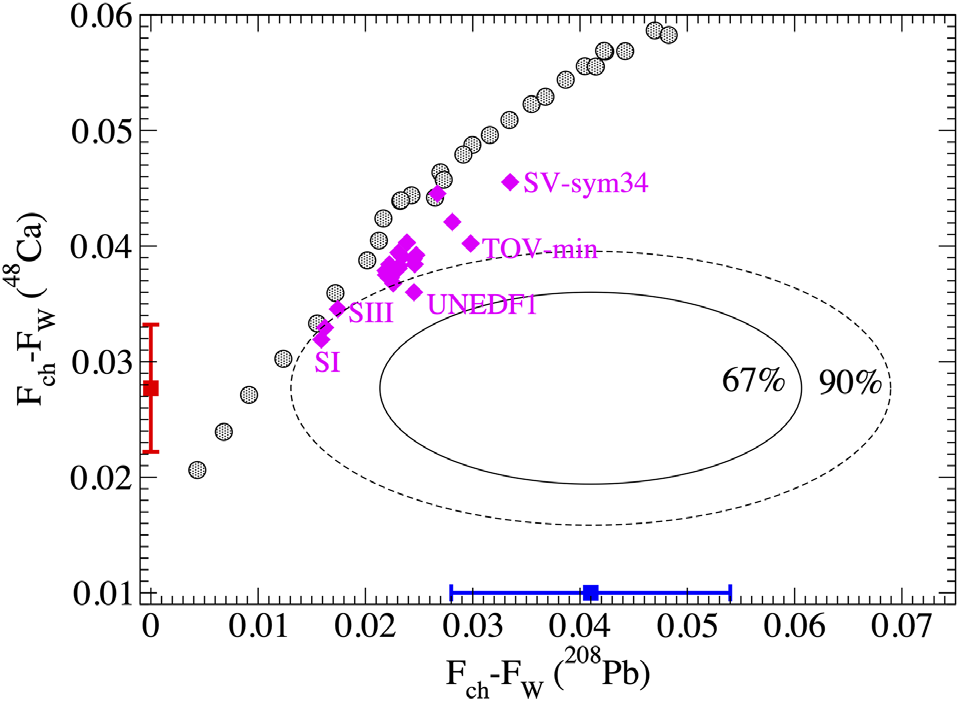
\includegraphics[width=0.49\linewidth]{FF_difference_Ca48_vs_Pb208}
    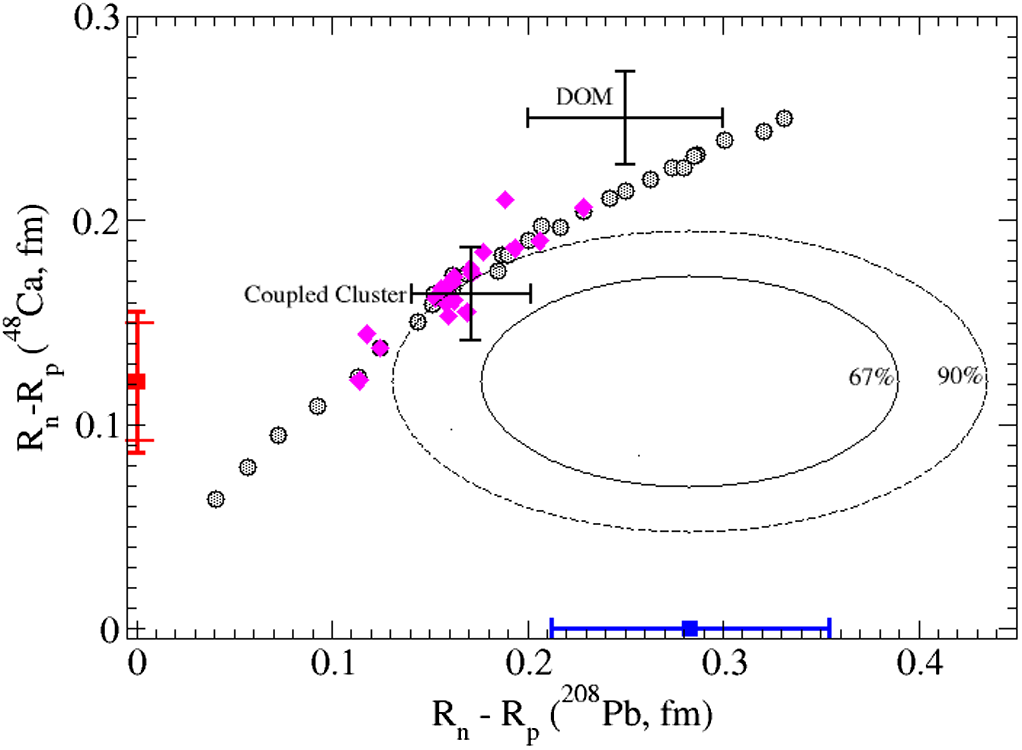
\includegraphics[width=0.49\linewidth]{neutron_skin_Ca48_vs_Pb208}
    \caption[FF and Rskin difference]
    {Experimental values and theoretical calculations of the FF difference (left)
    and the neutron skin thickness (right) of \Pb and \Ca. The two ellipses indicate
    the 67\% and 90\% probability intervals. The gray circles and magenta diamonds correspond
    to the DFT calculations using a range of relativistic and nonrelativistic density functionals,
    respectively. For clarity, only some of the functionals are labeled. 
    Additionally, Two ab-initio results:
    coupled cluster and dispersive optical model (DOM) are depicted in the 
    neutron skin thickness plot \cite{PhysRevLett.129.042501}.
    }
    \label{fig:pcrex_R_skin}
\end{figure}

\begin{comment}
% The strength of an EFT approach to the nuclear force lies in its power-counting capability. That is, theLagrangian of a theory with nucleons and pions can be expanded  order  by  order  in  terms  of  momentum  transfer  divided by a parameter that sets the momentum scale of the expansion
Various EFT models are based on an effective interaction Lagragian, for example,
FSUGold model has the following effective Lagrangian \cite{PhysRevLett.95.122501}:
\begin{equation}
    \begin{aligned}
	\CL_{\text{int}} = &\bar{\psi} \left[ g_s\phi - \left( g_v V_\mu + \frac{g_\rho}{2}\vec{\tau}\odot\vec{b}_\mu + \frac{e}{2}(1 + \tau_3) A_\mu \right)\gamma^\mu \right]\psi \\
	    & - \frac{\kappa}{3!}(g_s\phi)^3 - \frac{\lambda}{4!}(g_s\phi)^4 + \frac{\zeta}{4!}(g_v^2 V_\mu V^\mu )^2	\\
	    & + \Lambda_v(g_\rho^2\vec{b}_\mu\vec{b}^\mu)(g_v^2 V_\mu V^\mu)
    \end{aligned}
\end{equation}
This Lagrangian density describes interactions of the nucleon field $\psi$ to
various meson fields and their self-interactions. $\phi$ is a scalar.

The difference between different EFT models is just how many coupling they
include in their effective Lagrangian density. With the Lagrangian density,
one can calculate the properties of various nuclei, fitting predicted values
to experimental results to get a parameter set for the coupling constant in
the Lagrangian, which is called one model. Frequently used EFT models include
NL3 \cite{}, FSUGold \cite{} and 
\end{comment}

%%%%%%%%%%%%%%%%%%%%%%%%
\subsubsection{Limit of the Nuclear Landscape}

One straightforward application of nuclear DFT is to identify the limits of the nuclear
landscape. Every year, a varying number of new nuclides, ranging from just a few
to dozens, are discovered \cite{NEW_NULCIDES}. A clear theoretical guidance 
about the potential existence of neutron-rich nuclei will guide experimental 
efforts in the search for new rare isotopes, especially considering the challenges
posed by the low production rates of such neutron-rich nuclei.

The nuclear chart is defined by the boundaries known as the ``drip line'', 
which determines the maximum number of protons or neutrons for a given number 
of neutrons or protons. Specifically, across the drip line, the
separation energy of one proton ($S_{1p}$) or neutron ($S_{1n}$) 
or two protons ($S_{2p}$) or neutrons ($S_{2n}$) changes sign from positive to negative.
It is noteworthy that the neutron drip line is currently known only up to neon ($Z=10$), with the 
maximum number of neutrons being $N=24$ \cite{PhysRevLett.123.212501}. 
% https://physics.aps.org/articles/v15/177#c1

% \begin{figure}[!h]
%     \centering
%     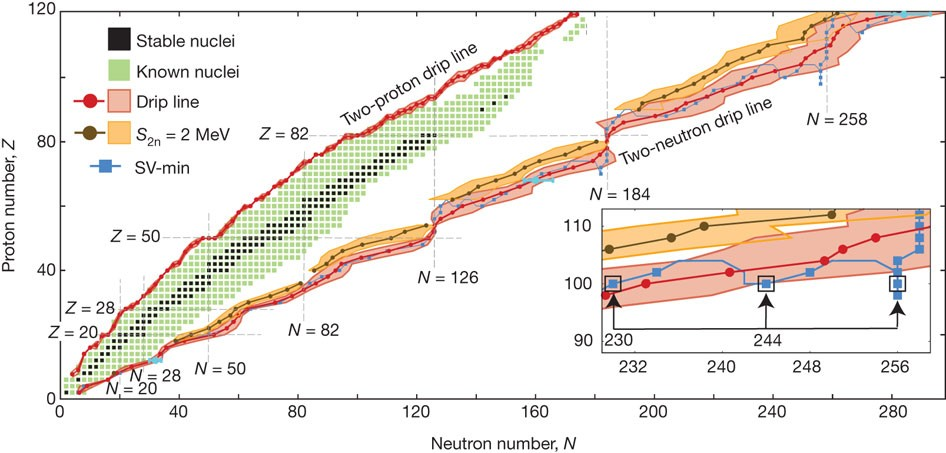
\includegraphics[width=0.8\linewidth]{nuclear_landscape_2012}
%     \caption{Nuclear landscape of even-even landscape as of 2012 \cite{Erler2012}.
%     The black .}
% \end{figure}

The neutron separation energy is defined as:
\begin{equation}
    \begin{aligned}
	S_{1n}(Z, N) &= E(Z, N-1) - E(Z, N) \\
	S_{2n}(Z, N) &= E(Z, N-2) - E(Z, N) \\
    \end{aligned}
\end{equation}
where $E$ is the binding energy. The same definition applies to protons.
A positive separation energy indicates that the nucleus is in a bound state, 
implying stability, while a negative value signifies an unstable state.
We are interested in both $S_{1n}$ and $S_{2n}$, rather than solely $S_{1n}$, because nuclei
with an even number of nucleons tend to be more stable compared to their neighboring
nuclei with an odd number of nucleons, due to the nucleonic superfluidity. 
At present, the estimate of the neutron drip line depends on the choice of 
theoretical models and associated parameterizations, as shown in Fig. \ref{fig:neutron_drip_line}. 
By incorporating the PREX-II and CREX results, we can constrain and refine
DFT models, consequently, enhancing the robustness of theoretical predictions
regarding the location of of the neutron drip line.
\begin{figure}[!h]
    \centering
    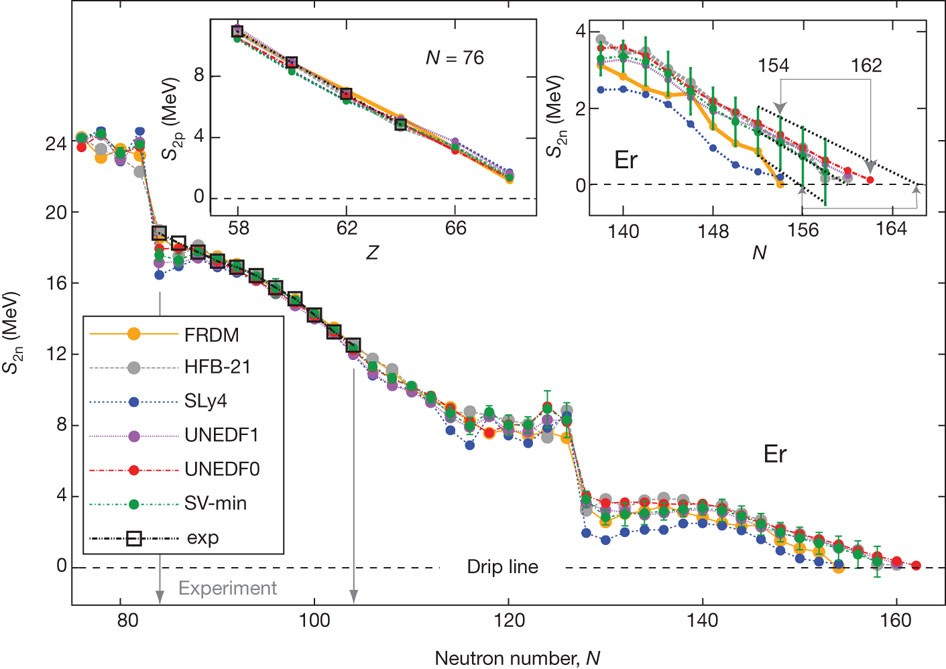
\includegraphics[width=0.8\linewidth]{drip_line}
    \caption[2-neutron separation energy]
    {Theoretical and experimental two-nucleon separation energies of
    even-even erbium isotopes \cite{Erler2012}. Dots represent DFT calculations
    and black squares correspond to experimental measurements.
    % These DFT models will be improved by our measurements, as shown in Fig.~\ref{fig:pcrex_R_skin}.
    }
    \label{fig:neutron_drip_line}
\end{figure}

%%%%%%%%%%%%%%%%%%%%%%%%
\subsubsection{Nuclear Saturation Density}
% for A > 20, B/A ~ constant (8 MeV)
The invariance of the binding energy per nucleon ($E_b/A$) with respect to $A$ implies that
the interaction between nucleons is proportional to $A$, rather than $A(A-1)$. 
This behavior indicates that nucleons saturate in space, leading to a nearly 
constant interior baryon density. 
A stricter definition of the saturation density
is the nucleon density at which the binding energy per nucleon is minimized.

While the concept of nuclear saturation is well-established, it is never directly observed.
\ca is the largest stable symmetric nucleus, it size is still too small to exhibit a nearly 
constant interior baryon density. For heavy nuclei, their charge densities have
been precisely measured, but no direct observation of any interior neutron density. 
PREX-II is the first experiment to provide a value of the average interior baryon density of 
a heavy nucleus with minimal reliance on theoretical models.

With the two-parameter Fermi function, the interior weak density is extracted 
from PREX-II result and determined to be:
% \cite{PhysRevC.102.044321}, we extract the weak charge saturation density.
\begin{equation}
    \rho_W^0({}^{208}\text{Pb}) = \frac{3Q_W}{4\pi c (c^2 + \pi^2 a^2)} 
    -0.0798 \pm 0.0038 \ (\text{exp}) \pm 0.0013 \ (\text{theo})\ \mathrm{fm}^{-3}
\end{equation}
where $Q_W$ is the total weak charge of \Pb nucleus.
\begin{equation}
    Q_W = -117.9 \pm 0.3
\end{equation}
% \begin{equation}
%     \rho^0_W = \frac{27 Q_{W}}{4\pi(5R^2_W - 4\pi^2 a^2)\sqrt{15R^2_W - 21\pi^2 a^2}}
% \end{equation}
Combining PREX-I and PREX-II results, $\rho_W^0$ is modified to be:
\begin{equation}
    \rho_W^0({}^{208}\text{Pb}) = -0.0796 \pm 0.0038 \mathrm{fm}^{-3}
\end{equation}
The uncertainty includes contributions from both experiment and theory.

With the well-measured interior charge density, the interior baryon density 
in \Pb is measured to be:
\begin{equation}
    \rho^0_b({}^{208}\text{Pb}) = 0.1482 \pm 0.0040\ \mathrm{fm}^{-3}
\end{equation}
The extracted density plot is shown in Fig.~\ref{fig:saturation_density}.

\begin{figure}[!h]
    \centering
    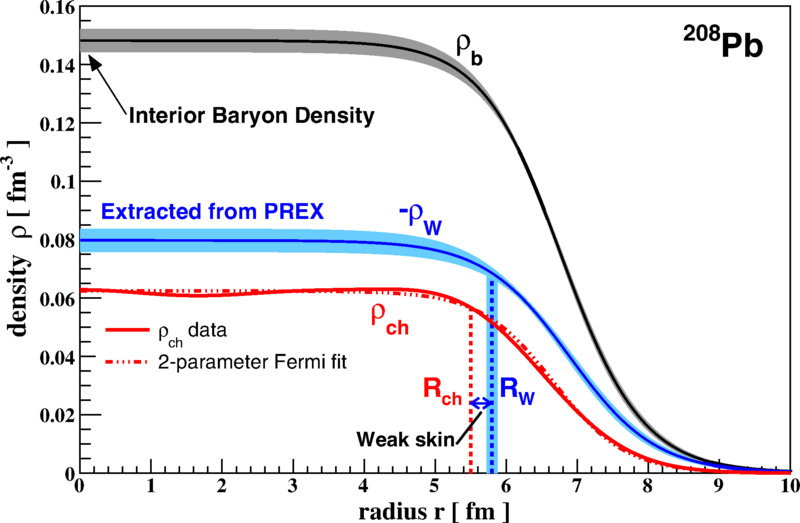
\includegraphics[width=0.6\linewidth]{prex_baryon_density}
    \caption{Density distributions for the EM charge (red), weak charge (blue) and
    baryon (black) in the \Pb nucleus \cite{PhysRevLett.126.172502}.}
    \label{fig:saturation_density}
\end{figure}

With the scale factor between the nuclear saturation density ($\rho_0$) and the interior
baryon density in \Pb ($\rho^0_b$) \cite{PhysRevC.102.044321}:
\begin{equation}
    f = \frac{\rho_0}{\rho^0_b} \approx 1.02 \pm 0.03
\end{equation}
The nuclear saturation density becomes:
\begin{equation}
    \rho_0 = f \times \rho_b^0 = 0.1510 \pm 0.0059 \ \mathrm{fm}^{-3}
\end{equation}
This value is fully consistent with $\rho_0 = 0.151 \pm 0.001 \ \mathrm{fm}^{-3}$ predicted
by a relativistic EDF calibrated using exclusively physical observables \cite{PhysRevC.90.044305},
and lower than the phenomenological estimate of $\rho_0 = 0.164 \pm 0.007 \ \mathrm{fm}^{-3}$ \cite{PhysRevLett.122.042501}
based on some selected density functionals.


\begin{comment}
%%%%%%%%%%%%%%%%%%%%%%%%%%%%%%%%%%%%%%%%%%%%%%%%
\subsection{Atomic Parity Violation Asymmetry}
Atomic parity violation is caused by the exchange of $Z^0$ boson between electrons
and the quarks in the nucleus, which interferes with the ``normal'' Coulomb interaction.

The exchange of a $Z^0$ boson is a parity violating effect and it causes the atomic states 
to acquire a small admixture of opposite-parity states. The effect is dominated by 
the admixture of P states into S states, $S \rightarrow S + \epsilon P$. 
In this case a parity-forbidden electric quadrupole E2 $S \rightarrow D$ transition 
is joined by an E1 parity non-conserving transition. The parity mixing effect is tiny, 
but it has been shown (Bouchiat \& Bouchiat, 1974) that it scales faster than $Z^3$, 
so the effect will be larger for heavier atoms.

Accuracy of atomic PV measurement is about 0.3\% (FIXME), which is important
for the test of the SM and the search for physics beyond the SM. A higher (0.1\%)
precision requires knowledge about the neutron radius better than 1\%. \cite{PhysRevC.46.2587}

\begin{equation}
    H_{PNC} \approx \frac{G_F}{2\sqrt{2}}\int [-N\rho_N(\vec{r}) + Z(1-4\sin^2\theta_W)\rho_P(\vec{r})] \phi_e^\dag \gamma^5\phi_e d^3r
\end{equation}

%%%%%%%%%%%%%%%%%%%%%%%%%%%%%%%%%%%%%%%%%%%%%%%%
\subsection{Coherent Neutrino Scattering off Nucleus}
\begin{equation}
    \frac{d\sigma}{dT} \approx \frac{G_F^2 M}{2 \pi}\frac{Q^2_W}{4}F^2(Q)\left ( 2 - \frac{MT}{E_\nu^2} \right)
\end{equation}
where E is the neutrino energy and T is the nuclear recoil energy. M being the
nuclear mass and $Q=\sqrt{2MT}$ is the momentum transfer.

\begin{itemize}
    \item neutrino floor for dark matter searches
    \item high precision determination of nuclei allow coherent neutrino 
	scattering to probe non-standard neutrino interactions.
\end{itemize}
\end{comment}

%%%%%%%%%%%%%%%%%%%%%%%%%%%%%%%%%%%%%%%%%%%%%%%%
\subsection{Neutron Stars}
As discussed in the introduction section, the measurement of the neutron skin 
thickness of \Pb and \Ca allows us to determine the density dependence of the symmetry energy,
which can then be used to constraint the size of a neutron star.

%%%%%%%%%%%%%%%%%%%%%%%%
\subsubsection{Multi-Messenger Measurements of the Neutron Star Radius}
NICER (Neutron star Interior Composition ExploreR) \cite{NICER} is a X-ray telescope that
can measure lightcurves of neutron stars (pulsars). Pulsars possess a hot-spot, which
is the magnetic pole of the neutron star. The observed light flux fluctuates 
based on the orientation of this hot-spot. When it faces the Earth, we observe the 
maximum flux,while minimum flux is observed when it points away from us. 
These variations occur due to the curvature of space caused by the neutron star. 
By analyzing the depth of the modulation in the light flux, one can infer the curvature of
space near the neutron star, which depends on the radius of the neutron star. 
This is how NICER measures the radius of a neutron star.
\begin{figure}[!h]
    \centering
    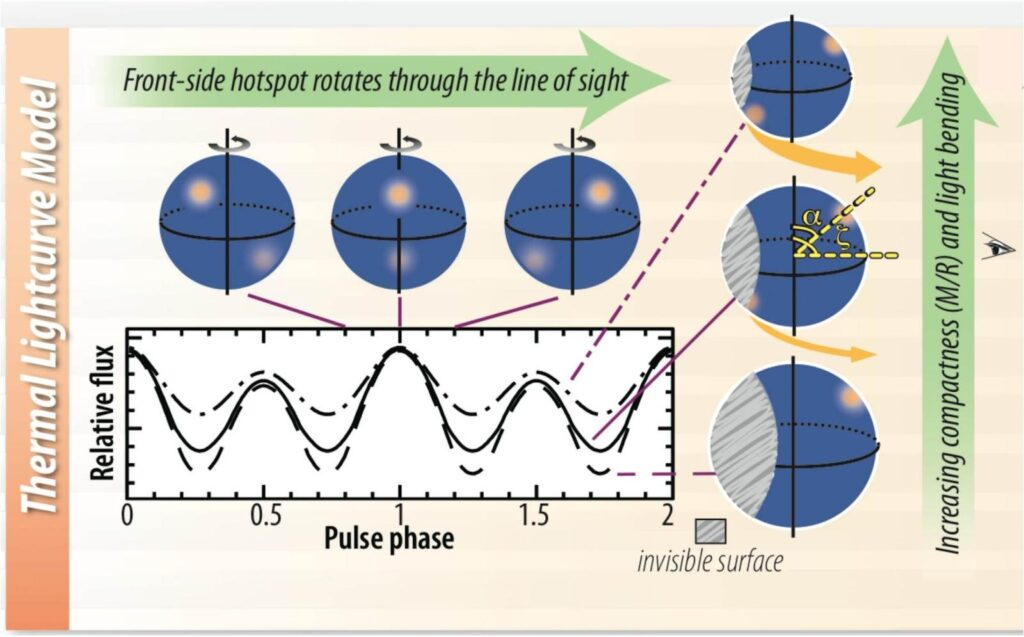
\includegraphics[width=0.6\linewidth]{pulsar_lightcurve}
    \caption[Light flux curve]{Modeling of the light flux from a neutron star. The three curves
    in the flux panel corresponding to the three neutron stars to the right
    with different compactness (mass/radius).
    % https://n3as.berkeley.edu/p/neutron-stars-sound-speed-dense-qcd/
    }
\end{figure}

One can measure the size of a neutron star through the gravitational waves as well.
The famous LIGO-Virgo event, GW170817 \cite{PhysRevLett.119.161101}, 
observed the gravitational wave emission from a binary neutron star merger. 
In such a binary system, the neutron star experiences deformation
due to the tidal force exerted by the other body, this property is described by the
tidal deformability (quadrupole polarizability):
\begin{equation}
    \Lambda = \sum_f \frac{|\bra{f}r^2Y_{20}\ket{i}|^2}{E_f - E_i} \propto R^5 
\end{equation}
Tidal deformability can be probed by detection of the gravitational waves produced
by the binary system.
LIGO observation of GW170817 sets an upper limit on $\Lambda$ of a typical 1.4 $M_\odot$
neutron star\cite{PhysRevLett.121.161101}. 
\begin{equation}
    \Lambda_{1.4} = 190^{+390}_{-120}
\end{equation}
It favors a smaller deformability ($<580$) and consequently a smaller neutron star radius ($<13$~km)

\begin{figure}[!h]
    % page 12 of https://indico2.riken.jp/event/3082/contributions/17269/attachments/10634/15080/PREX2SPIN2021_DonJones.pdf
    \centering
    \begin{tikzpicture}
	\begin{scope}
	    \node[anchor=south west, inner sep=0] (image) at (0, 0)
	    { 
		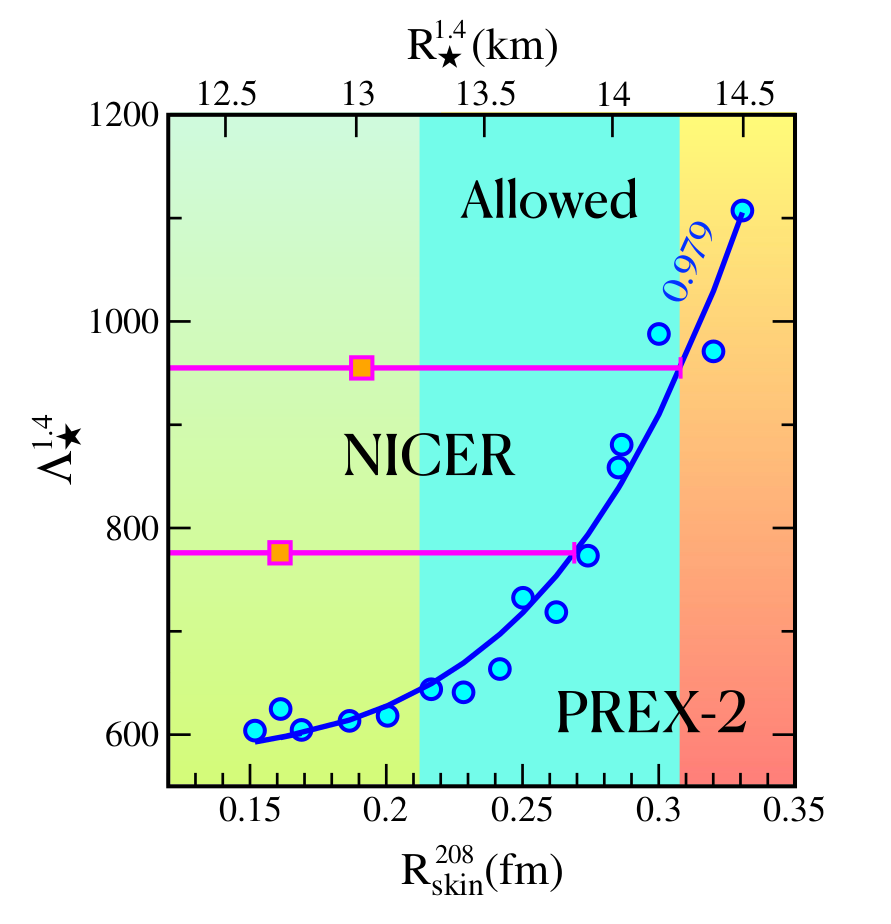
\includegraphics[width=0.65\linewidth]{neutron_star_radius}
	    };
	    \begin{scope}[x={(image.south east)}, y={(image.north west)}]
		\draw[very thick, dashed, red] (0.19, 0.19) -- ++(0.21, 0) node [right] {\textbf{LIGO 90\% CL}};
		\draw[very thick, dashed, red] (0.89, 0.19) -- ++(-0.21, 0);
	    \end{scope}
	\end{scope}
    \end{tikzpicture}
    \caption[Tidal deformability versus Rskin]
    {Tidal deformability of a 1.4 $M_\odot$ neutron star versus its radius (upper X-axis)
    and the neutron skin thickness of \Pb (lower X-axis). Blue dots represent theoretical
    predictions from a set of EDFs, while the blue line is a fit to these dots. 
    PREX-2 in the plot refers to the combined result of PREX-I and II.
    The light blue region corresponds to the radius range allowed by both NICER and
    PREX-2 \cite{PhysRevLett.126.172503}}.
    \label{fig:neutron_star_radius}
\end{figure}

Observables of a 1.4 $M_\odot$ neutron star extracted from various experiments
are shown in Fig.~\ref{fig:neutron_star_radius}. We see that the combined PREX 
measurement is consistent with the NICER result, while in mild tension with
the LIGO observation.
% PREX-II result suggests EoS is still at low density while NICER and LIGO observations
% indicate that EoS is soft at high density.
% The softening of EoS with density could strongly suggest a transition to an
% exotic high density phase such as quark matter, strange matter, color superconductor
% and kaon condensate

\begin{comment}
    \item Dipole polarizability of an atom $\sim R^3$
	$$ \kappa = \sum_f \frac{|\bra{f}rY_{10}\ket{i}|^2}{E_f - E_i} \propto R^3 $$
    \item Tidal deformability (quadrupole polarizability) of a neutron star scales as $R^5$
	$$ \Lambda = \sum_f \frac{|\bra{f}r^2Y_{20}\ket{i}|^2}{E_f - E_i} \propto R^5 $$
    \item Next generation observer: cosmic explorer (https://arxiv.org/abs/2109.09882)
	can accurately determine deformability of neutron stars
\end{comment}

%%%%%%%%%%%%%%%%%%%%%%%%
\subsubsection{Direct Urca Process}
% some neutron stars seem too cold
The direct Urca processes are neutrino emission processes: 
\begin{equation}
    \begin{gathered}
	n \rightarrow p + e^- + \bar{\nu}_e \\
	p + e^- \rightarrow n + \nu_e \\
    \end{gathered}
\end{equation}
which may explain the rapid cooling of some neutron stars \cite{Haensel1995}. 

The rate of the direct Urca process depends on the proton fraction present in the core
of a stellar object. This proton fraction, in turn, is controlled by the density dependence of 
the symmetry energy \cite{PhysRevLett.120.182701}. Therefore, we can gather insights
into the threshold density for the direct Urca process from the measurement of $R_{\text{skin}({}^{208}\text{Pb})}$,
as shown in Fig.~\ref{fig:DUrca}. 
In particular, a higher neutron skin thickness observed in \Pb corresponds to a
lower threshold mass (density) required for the occurence of the direct Urca process. 
Our measurement of $R_{\text{skin}}({}^{208}\text{Pb}) = 0.283\ \mathrm{fm}$
suggests a threshold mass of $M_\bigstar \approx 0.85 M_\odot$ and a corresponding
threshold density of $\rho_\bigstar \approx 0.24\ \mathrm{fm}^{-3}$.
\begin{figure}[!h]
    \centering
    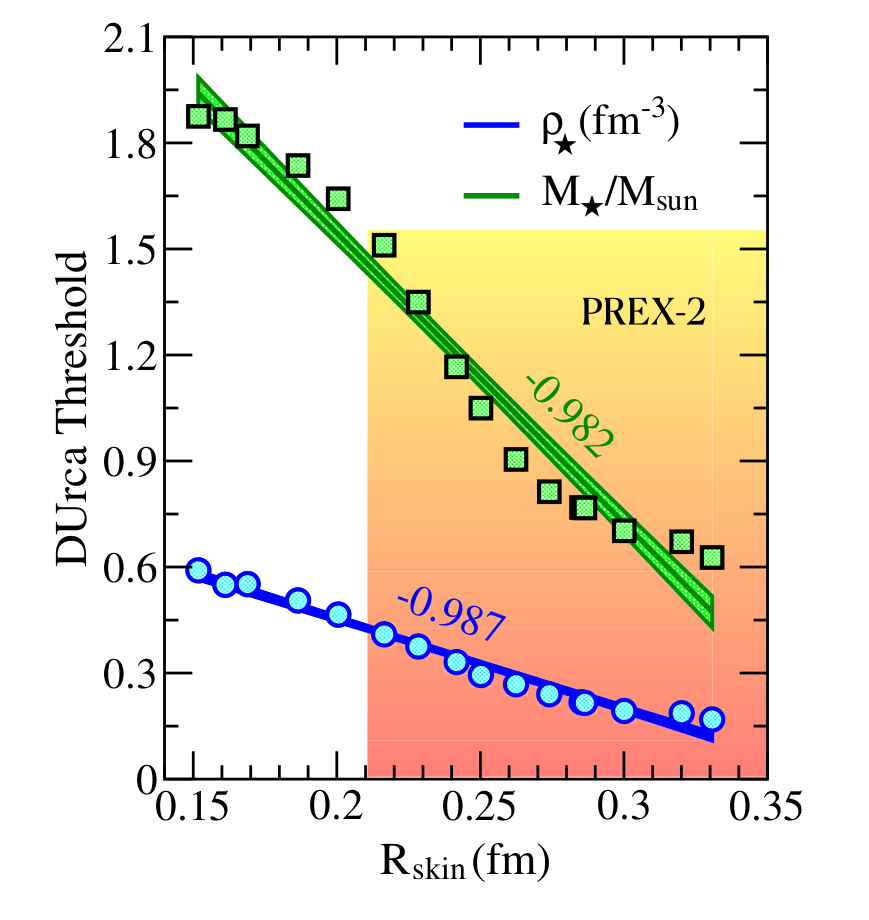
\includegraphics[width=0.5\linewidth]{UCRA_vs_R_skin}
    \caption[Direct Urca threshold]
    {The direct Urca threshold densities (blue dots) and corresponding 
    stellar mass (green dots) versus the neutron skin thickness of \Pb. PREX-2 
    in the plot refers to the combined result of PREX-I and II.
    The shaded area represents the combined PREX 1-$\sigma$ confidence region \cite{PhysRevLett.126.172503}.}
    \label{fig:DUrca}
\end{figure}

%%%%%%%%%%%%%%%%%%%%%%%%%%%%%%%%%%%%%%%%%%%%%%%%%%%%%%%%%%%%%%%%%%%%%%%%
\section{Future Outlook}
Parity-violating electron scattering experiments continue to advance and thrive
in their development.
Several PVES experiments have been proposed to investigate different aspects of EW
interactions, including MOLLER \cite{MOLLER} and SoLID \cite{SoLID} at JLab, 
as well as P2 and MREX at Mainz \cite{Becker2018}.

%%%%%%%%%%%%%%%%%%%%%%%%
\subsubsection{Measurement Of a Lepton Lepton Electroweak Reaction (MOLLER)}
As a test of the SM, the weak mixing angle ($\sin^2\theta_W$) is of great importance 
and have been measured by different experiments, as shown in Fig.~\ref{fig:weak_mixing_angle}.

\begin{figure}[!h]
    \centering
    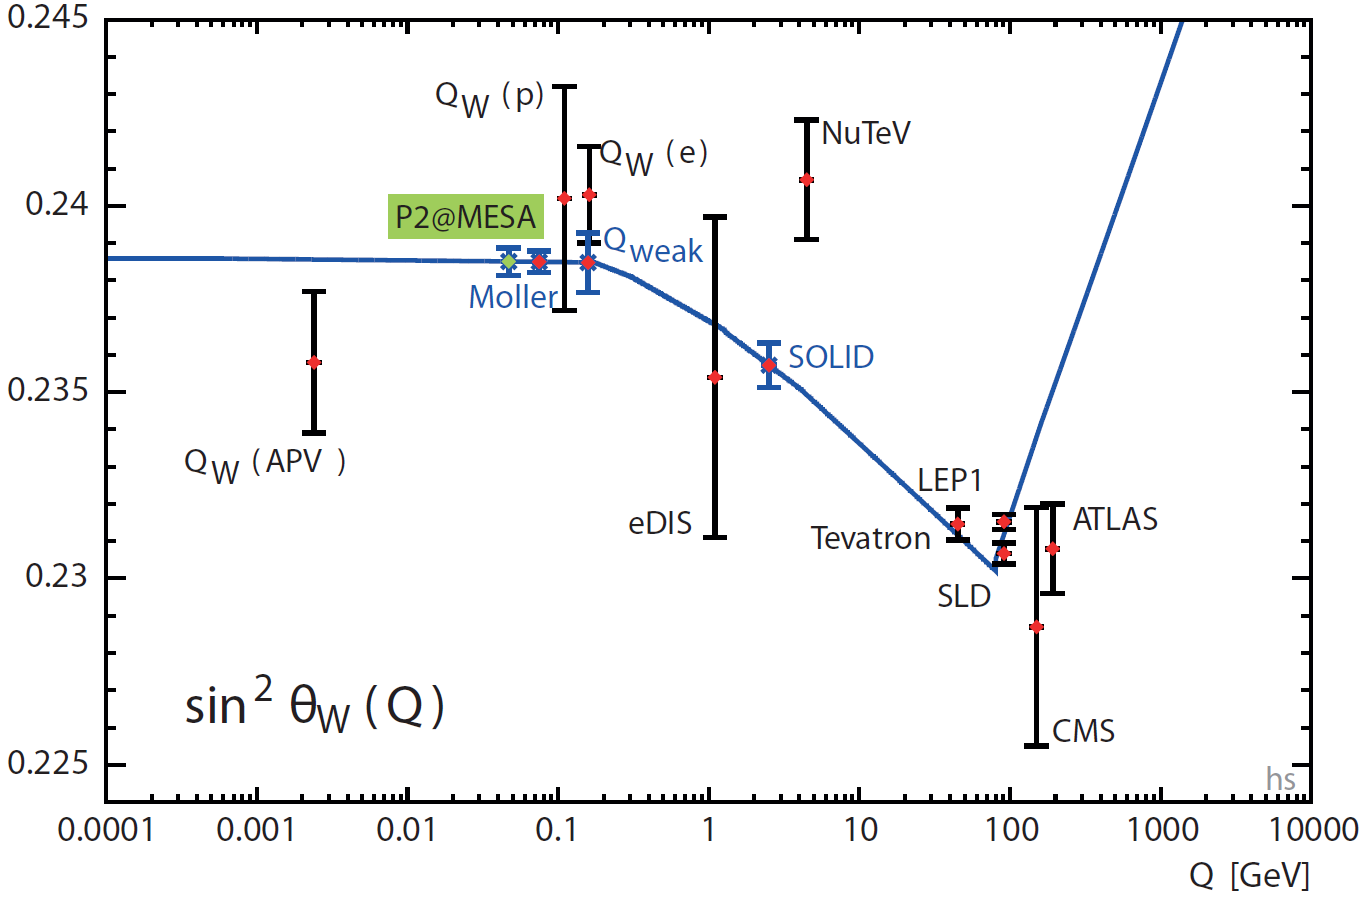
\includegraphics[width=0.5\linewidth]{weak_mixing_angle}
    \caption{Various (proposed) measurements of the running weak mixing angle
    along the energy scale. }
    \label{fig:weak_mixing_angle}
\end{figure}

The proposed MOLLER experiment at JLab, as a successor to the SLAC E158 experiment \cite{PhysRevLett.95.081601},
aims to significantly improve the E158 result by a factor of five, which will be a 2.4\%
relative uncertainty in $Q_W^e$, corresponding to a 2.1\% relative uncertainty
in the measurement of $\CA_{\text{PV}}$ ($33 \pm 0.7$~ppb).
This low energy precision frontier experiment will produce the most precise 
measurement of $\sin^\theta_W$ over the next decade. The high precision of the measurement
enables sensitivity to the interference between the known EM amplitude and any
possible new neutral currents. This sensitivity allows for probing new particles 
beyond the Higgs mass, reaching up to a scale of $\sim 27$~TeV.

%%%%%%%%%%%%%%%%%%%%%%%%
\subsubsection{Solenoidal Large Intensity Device (SoLID)}
SoLID, another proposal at JLab, focus on probing the parity-violating effect in deep inelastic
scattering (PVDIS). SoLID refers to a new spectrometer of large angular and momentum
acceptance, meanwhile, it can handle high luminosity. This new apparatus will
measure $\CA_{\text{PV}}$ to a very high precision of about 0.5\% over a wide
range of Bjorken x and $Q^2$. The SoLID PVDIS project will employ several
different targets. Deuterium will provide a new measurement of the weak mixing angle
in the medium energy region, as shown in Fig.~\ref{fig:weak_mixing_angle};
with a hydrogen target, the proton $d/u$ ratio can be measured and a heavy
nucleus like \Pb allows the study of the flavor dependence of the EMC effect \cite{Aubert:142300}.


%%%%%%%%%%%%%%%%%%%%%%%%
\subsubsection{P2 and MREX}
While the MOLLER experiment aims to provide the most precise measurement of the
weak mixing angle, the most precise measurement of the weak charge will be carried
out by the P2 experiment at Mainz.
P2 will measure the weak charge of the proton, a quantity that was previously
measured by the Qweak experiment at JLab \cite{PhysRevLett.111.141803}.
Compared to Qweak, P2 plans to improve the measurement precision by a factor of three,
aiming for a 0.15\% precision in the determination of the weak mixing angle.
Similar to MOLLER, the high precision achieved by P2 enables an indirect search 
for new physics beyond the SM, up to a mass scale of 50~TeV.

Finally, the Mainz radius experiment (MREX) will measure the neutron skin thickness of \Pb
again, at a lower $q$ value and will improve the PREX result to a higher precision
of 1.4\% \cite{Becker2018}.

\bigskip
Indeed, the advancements in experimental techniques within the field are highly encouraging. The pursuit of higher precision in measuring the parity-violating asymmetry by next-generation PVES experiments positions them as promising candidates for exploring new physics beyond the Standard Model.

These experiments not only have the potential to discover new phenomena and particles but also significantly contribute to our understanding of nuclear physics. By achieving higher precision in PVES measurements, researchers can gain improved insights into nuclear structure, potentially uncovering new aspects that were previously unknown. This continuous drive for precision and the search for new physics create an exciting frontier for scientific exploration in both particle physics and nuclear physics. It is an area where new discoveries and breakthroughs are eagerly anticipated, enriching our understanding of the fundamental nature of matter and the universe.
